\chapter{光栅图像}

大多数CG(computer graphics)图片在某种光栅显示器上呈现给用户。光栅显示器以矩形像素阵列的方式呈现图片。一个常见的例子是平板显示器或平板电视,它们有一个由微小的发光像素组成的矩形阵列,每个发光像素都可以被设置成不同的颜色从而得到任何想得到的图像。不同的颜色是通过混合不同强度的红、绿、蓝光实现的。大多数打印机,如激光打印机和喷墨打印机,也是光栅设备。它们以扫描为基础:实际上没有由像素组成的物理网格,但图像是通过在网格上选定的点上沉积墨水而按顺序铺设的。

\marginpar{
  \begin{center}
    \begin{note}\\
      像素(Piexl)是图像元素(picture element)的简称。
    \end{note}
  \end{center}
}

\marginpar{
  \begin{center}
    \begin{note}\\
      打印机的颜色更复杂,涉及至少有四种颜料的混合物。
    \end{note}
  \end{center}
}

光栅也被普遍应用到了图像输入设备上。一块数码相机包括一个由光感像素网格组成的图像传感器,每个光感像素都能记录颜色和落在其上的光线强度。一台桌面扫描器包括一个由像素组成的线性阵列,它每秒横向扫描页面并不断记录来产生像素网格。

由于光栅在设备中相当普遍,光栅图像是储存、处理图像的最常见方式。一幅光栅图像只是一个储存了每个像素的像素值(通常是一个由三个数字表示的颜色,分别代表红、绿、蓝)的二维数组。内存中存储的光栅图像可通过被存储图像的每个像素值来一一控制显示器上单个像素的颜色从而被显示出来。

\marginpar{
  \begin{center}
    \begin{note}\\
      也可能是因为光栅图像如此便利以至于光栅设备如此普遍。
    \end{note}
  \end{center}
}

但我们并不总是以这种方式显示图片。 我们可能想要改变图像的大小和朝向,修正颜色,甚至将图像显示在运动的三维空间平面上。即使在电视上,显示器也很少会有和图像相同的像素数量。诸如此类的考虑打破了图像像素和显示像素之间的直接联系。最好把光栅图像看作是对要显示的图像的独立设备描述,而把显示设备看作是接近该理想图像的一种方式。

除了使用像素阵列,还有其他方式描述图像。矢量图像通过存储图形的描述来绘制图像——由线条和曲线围成的色彩区域——不包含对特定像素网格的引用。本质上,这相当于存储如何显示图像的说明而不是存储需要显示的像素。矢量图像的主要优势在于他们是分辨率独立的,因此在高分辨率设备上也具有很好的显示效果。而相对应的,其缺点在于在显示前图像需要被栅格化。矢量图像经常用于文本、图表、机械制图、对清晰度和精确度要求较高的应用场合以及不需要摄影图像和复杂阴影的场景。

在这个章节,我们讨论光栅图像和光栅显示器的基础,特别需要注意标准显示器的非线性问题。当我们在后面的章节中讨论计算图像时,像素值如何与光强度建立联系的细节是很重要的并需要牢记于心。

\marginpar{
  \begin{center}
    \begin{note}\\
      或者说:你需要知道图像中这些数值的真正含义。
    \end{note}
  \end{center}
}

\section{光栅设备}

在讨论抽象的光栅图像之前,了解使用这些图像的一些具体设备的基本操作是很有意义的。一些熟悉的光栅设备可以被归入一个简单的层次结构中:

\begin{itemize}
  \item 输出
        \begin{itemize}
          \item 显示器
                \begin{itemize}
                  \item 透射式显示器:液晶显示器(LCD)
                  \item 自发光式显示器:发光二极管(LED)显示器
                \end{itemize}
          \item 打印
                \begin{itemize}
                  \item 二值图像:喷墨打印机
                  \item 连续色调(continuous-tone)图像:热升华打印机
                \end{itemize}
        \end{itemize}
  \item 输入
        \begin{itemize}
          \item 二维阵列传感器:数码相机
          \item 一维阵列传感器:平板扫描仪
        \end{itemize}
\end{itemize}

\subsection{显示器}

目前的显示器,包括电视和数字电影放映机以及计算机显示器和投影仪,几乎普遍基于固定的像素阵列。它们可以分为自发光式显示器,它使用直接发射可控光量的像素,和透射式显示器,其中像素本身不发光,而是改变它们允许通过的光量。透射式显示器需要光源来照亮它们:在直视型显示器中,光源是阵列后面的背光;在投影仪中,光源是一盏灯,它发出的光穿过阵列后投射到屏幕上。而自发光式显示器便是其自身的光源。

\marginpar{
  \begin{center}
    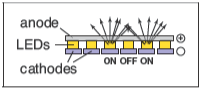
\includegraphics[width=0.25\textwidth]{3.1.png}
    \captionof{figure}{发光二极管(LED)显示器的运行机制。}
  \end{center}
}

发光二极管(LED)显示器是自发光式显示器的一个例子。每个像素由一个或多个LED组成,这是一种基于通过电流强度决定发光亮度的半导体设备(基于有机/无机半导体)(图3.1)。

\marginpar{
  \begin{center}
    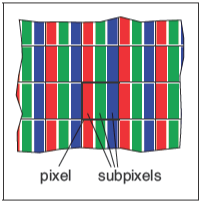
\includegraphics[width=0.25\textwidth]{3.2.png}
    \captionof{figure}{组成平板显示器中单个像素的红、绿、蓝子像素。}
  \end{center}
}

彩色显示器上的像素被细分为3个独立控制的子像素,一个红色、一个绿色、一个蓝色,每个LED都由不同材料组成从而发出不同颜色的光(图3.2)。当从一定距离外观看显示器时,眼睛无法分开每个独立的子像素,最后感知到的颜色便是红、绿、蓝三色混合成的颜色。

液晶显示器(LCD)是透射式显示器的一个例子。液晶是一种材料,其分子结构使其能够旋转通过它的光的偏振,并且旋转的程度可以通过施加的电压来调节。LCD像素(图3.3)后面有一层偏振膜,因此它被偏振光照亮——让我们假设光是水平偏振的。

\begin{figure}[htb]
  \centering
  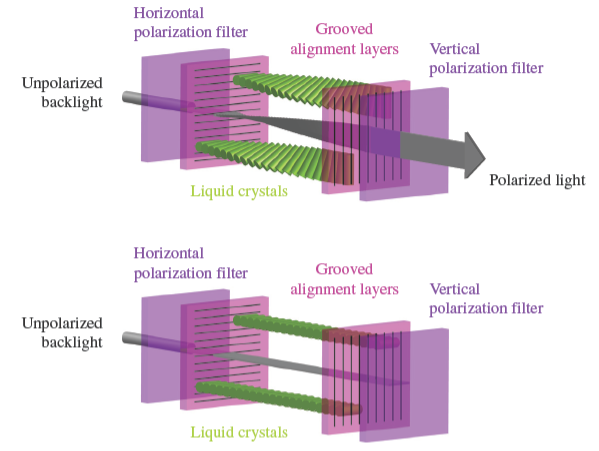
\includegraphics[width=1.0\textwidth]{3.3.png}
  \caption{上图是一个处于开启状态的LCD显示器像素,其中液晶单元旋转光线的偏振方向,因此光线能通过前端偏振片。下图是一个处于关闭状态的LCD显示器像素,其中前端偏振片阻挡了所有通过后端偏光片的光线。图由Reinhard, Khan, Akyilz and Johnson(2008)提供。}
\end{figure}

\marginpar{
  \begin{center}
    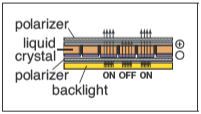
\includegraphics[width=0.25\textwidth]{3.4.png}
    \captionof{figure}{液晶显示器(LCD)的运行机制。}
  \end{center}
}

像素前的第二层偏振膜只传导垂直偏振光。如果液晶层两端施加电压至不改变偏振方向,则所有光都被阻挡且像素处于“关闭”状态(最小光强度)。如果电压被设置以让液晶层改变偏振方向至90度,则所有从像素后方进入的光都将从前端逃离,此时像素处于完全“开启”状态(具有最大光强度)。 而中等的电压会部分旋转偏振角,这样前端偏振片会阻挡部分光线,最终产生的光强度介于最大值与最小值之间(图3.4)。就像彩色LED显示器一样,彩色LCD显示器的像素中也包含红、绿、蓝子像素,实质上是三个独立的、覆盖有红、绿、蓝三种颜色过滤器的像素。

\marginpar{
  \begin{center}
    \begin{note}\\
      显示器的分辨率有时被叫做“本地分辨率”因为许多显示器都可以通过内置转换处理其他分辨率的图片。
    \end{note}
  \end{center}
}

任何形式的有固定像素阵列的显示器——包括以上这些或其他技术——都有一个由阵列大小决定的基础的固定分辨率。对于显示器或图像,分辨率仅仅意味着像素阵列的尺寸:如果桌面显示器有1920*1200的分辨率,那么它总共有2304000个像素分布在1920列和1200行的像素阵列中。

\subsection{打印设备}

在纸上永久记录图像的过程与在显示器上短暂地显示图片相比有许多限制。在印刷中,颜料被分布于纸上或其他打印媒介上,当光从纸上反射后便能形成想要的图案。打印机是类似于显示器的光栅设备,但许多打印机只能打印二值图像,即每个网格位置要么沉积颜料,要么不沉积,没有可能的中间值。

\marginpar{
  \begin{center}
    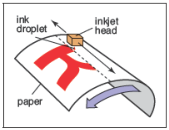
\includegraphics[width=0.25\textwidth]{3.5.png}
    \captionof{figure}{喷墨打印机的运行机制。}
  \end{center}
}

喷墨打印机(图3.5)是一种通过扫描形成光栅图像的设备。喷墨打印头容纳了含有颜料的液体墨水,并能通过电子控制将墨水以微小墨滴的形式喷出。喷墨头在纸上横向移动,当它经过应该接受墨水网格位置时便会将墨滴喷射出;想要保持空白的位置则不会喷射墨滴。喷墨头每次扫描(sweep)之后,纸张都会略微前移,随后网格的下一行被喷射到纸上。彩色打印机使用数个打印头,每个喷头喷射一种不同的颜色的墨水,因此每个网格位置可接受任何由不同颜色的墨滴混合成的颜色。由于所有墨滴都一样,一台打印二值图像的喷墨打印机在每个网格格点上要么有墨滴要么没有墨滴,没有中间的色度(shade)。

\marginpar{
  \begin{center}
    \begin{note}\\
      也存在连续喷墨打印机,它以连续的螺旋路径打印包裹在旋转的滚筒周围的纸张,而不是来回移动打印头。
    \end{note}
  \end{center}
}

喷墨打印机没有物理像素阵列,其分辨率由墨滴的尺寸以及喷墨头每次扫描后纸张前进的距离决定。许多喷墨打印机的打印头中有多个喷嘴,允许其在一次横向移动中完成多次扫描,但最终是由纸张前移距离决定行距而非喷嘴间距。

\marginpar{
  \begin{center}
    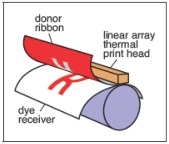
\includegraphics[width=0.25\textwidth]{3.6.png}
    \captionof{figure}{热敏染料转印打印机的运行机制。}
  \end{center}
}

热敏染料转印工艺是连续色调印刷工艺的一个例子,这意味着可以在每个像素上沉积不同量的染料 - 它不像喷墨打印机那样全有或全无(图3.6)。将含有彩色染料的供体色带压在纸张(或染料接收器)与包含加热组件线性阵列的打印头之间,图片的每列像素分配一个加热组件。当纸张和色带经过打印头时,加热组件通过打开和关闭状态来在需要染料的区域加热色带,使染料从色带扩散到纸张。对几种染料中的每一种重复此过程。由于较高的温度会导致更多的染料被转印,因此可以控制在每个网格位置沉积的每种染料的量,从而产生连续的颜色范围。打印头中加热组件的数量在页面横向方向上确定了固定的分辨率,但沿页面的分辨率由加热、冷却速率与纸张速度的关系决定。

\marginpar{
  \begin{center}
    \begin{note}\\
      术语“DPI”经常被用于表达“PPI”的含义,但“DPI”应被用于涉及二值设备的情况,而“PPI”应被用于涉及连续色调设备的情况。
    \end{note}
  \end{center}
}

与显示器不同,打印机的分辨率是根据像素密度而不是像素总数来描述的。因此,如果热敏染料转印打印机的打印头上每英寸的加热元素间距为300,则其整个页面的分辨率为每英寸300个像素(ppi)。如果选择沿页面的分辨率相同,我们可以简单地说打印机的分辨率为300ppi。将点放在每英寸 1200 个网格点上的喷墨打印机被描述为分辨率为每英寸1200个点(dpi)。由于喷墨打印机是二值设备,因此至少出于两个原因,它需要更精细的网格。由于边缘是突兀的黑/白边界,因此需要非常高的分辨率来避免出现锯齿(stair-stepping/aliasing)(详见第9.3节)。打印连续色调图像时,需要高分辨率通过打印称为半色调的不同密度点图案来模拟中间色。

\subsection{输入设备}

\marginpar{
  \begin{center}
    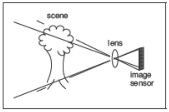
\includegraphics[width=0.25\textwidth]{3.7.png}
    \captionof{figure}{数码相机的运行机制。}
  \end{center}
}

光栅图像不能凭空产生,并且任何不是由算法产生的图像都需要通过光栅输入设备记录(通常是相机或扫描仪)。即使是3D场景渲染而成的图像也通常使用照片作为纹理映射(详见第11章)。光栅输入设备需要对每个像素进行光记录,并且(就像输出设备一样)它们通常基于传感器阵列。

\marginpar{
  \begin{center}
    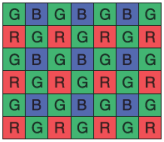
\includegraphics[width=0.25\textwidth]{3.8.png}
    \captionof{figure}{许多彩色数字相机使用类似于上图所示的“拜尔马赛克”(Bayer mosaic)的色彩滤镜阵列。每个像素记录红光、绿光或蓝光。}
  \end{center}
}

数码相机就是一种二维阵列输入设备。相机中的图像传感器是一个拥有光敏像素网格的半导体设备。两种常见的阵列类型是电荷耦合元件(CCDs, charge-coupled devices)和互补金属氧化物半导体(CMOS, complimentary metal-oxide-semiconductor)图像传感器。相机的镜头将要被照相的景物的图片传感器上,然后每个像素记录落在其上的光能,最终产生构成输出图像的数字(图3.7)。就像颜色通过红、绿、蓝子像素进行显示一样,许多相机通过使用“色彩滤镜阵列”(color-filter array)或“马赛克”(mosaic)来让每个像素只能感知红光、绿光或蓝光,而图像处理软件则在称为“去马赛克”(demosaicking)的过程中填充缺失值(图3.8)。

\marginpar{
  \begin{center}
    \begin{note}\\
      买相机的人通常使用兆(mega)来表示$10^6$,而不是兆字节(megabytes)代表的数量级$2^{20}$。
    \end{note}
  \end{center}
}

其他相机使用3个独立阵列或阵列中的3个独立层级来在每个像素上记录独立的红、绿、蓝值,直接产生可用的彩色图片而无需更进一步地处理。相机分辨率由阵列中像素的固定数量决定,并且通常被描述为像素总数:一台阵列有3000列和2000行的相机产生分辨率3000*2000的图像,其中有六百万像素,称为“6兆像素”(MP, megapixel)相机。需要注意马赛克传感器并不记录一幅完整的图像,因此记录相同像素数但具有独立红色、绿色和蓝色记录值的相机比使用马赛克传感器的相机记录更多有关图像的信息。

\marginpar{
  \begin{center}
    \begin{note}\\
      由于许多扫描仪可以通过内置转换产生其他分辨率的图像,扫描仪的分辨率有时被称为“光学分辨率”。
    \end{note}
  \end{center}
}

平板扫描仪也记录每个像素网格的红色、绿色和蓝色值。但与热敏染料转印打印机一样,它使用一维阵列横扫正在被扫描的页面,每秒进行多次记录(图3.9)。页面的横向分辨率由阵列的尺寸确定,并且页面的纵向分辨率由记录频率和扫描头移动的速度确定。彩色扫描仪具有 $3\times n_x$ 阵列,其中$n_x$是页面的横向像素数,包括三行由红色、绿色和蓝色滤镜覆盖(的子像素)。在记录三种颜色的时间之间有适当的延迟,这允许在每个网格点进行三个独立的颜色记录。与连续色调打印机一样,扫描仪的分辨率以每英寸像素数 (ppi) 为单位进行报告。

有了这些关于我们的图像来自哪里以及它们将去哪里的具体信息,我们现在将更抽象地讨论图像,就像我们在图形算法中使用它们一样。

\marginpar{
  \begin{center}
    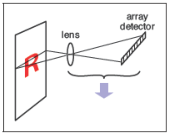
\includegraphics[width=0.25\textwidth]{3.9.png}
    \captionof{figure}{平板扫描仪的运行机制。}
  \end{center}
}

\section{图像、像素和几何}

我们知道光栅图像是一个大的像素阵列,每个像素都存储了图像在该网格点的信息。我们也看到了数种输出设备如何处理我们发给它的图像,以及输入设备如何从物理世界中由光形成的图像中获取它们。但是对于计算机中的计算,我们需要一个独立于任何设备细节的方便抽象,我们可以用它来推理如何生成或解释存储在图像中的值。

当我们记录或再现图像时,它们采取光能的二维分布的形式:显示器发出的光作为位置在显示器表面上的函数;落在相机图像传感器上的光作为传感器平面上位置的函数;反射率(reflectance),或反射光的分数(相对于吸收的),作为一张纸上位置的函数。因此,在物理世界中,图像是在二维区域(几乎总是矩形)上定义的函数。因此,我们可以将图像抽象为函数
\marginpar{
  \begin{center}
    \begin{note}\\
      “像素不是小正方形!”  ——Alvy Ray Smith(1995)
    \end{note}
  \end{center}
}
\[
  \begin{aligned}
    I(x,y):R\rightarrow V,
  \end{aligned}
\]
其中$R\subset \mathbb{R} ^2$是一个矩形区域,而$V$是一个可能像素值的集合。最简单的例子是一个理想化的灰度图像,其矩形中的每个点只有亮度(而不是颜色),因此我们可以说$V=\mathbb{R}^{+}$(非负实数)。一幅理想化的彩色图像,每个像素都有红色、绿色、蓝色值,有$V=(\mathbb{R}^{+})^3$。我们将在下一小节讨论$V$的其他可能性。

\marginpar{
  \begin{center}
    \begin{note}\\
      有没有其他不是矩形的光栅设备?
    \end{note}
  \end{center}
}

光栅图像与连续图像的这个抽象概念有什么关系?从具体的例子来看,照相机或扫描仪的一个像素是对该像素周围某个小区域的图像平均颜色的记录。一个具有红、绿、蓝子像素的显示器像素被设计成图像在像素面上的平均颜色由光栅图像中的相应像素值控制。在这两种情况下,像素值是图像颜色的局部平均值,它被称为图像的点样本。换句话说,当我们找到一个像素的值$x$时,它意味着“这个网格点附近的图像的值是$x$”。 图像作为函数的采样表示的想法将在第十章中进一步探讨。

\begin{figure}[htb]
  \centering
  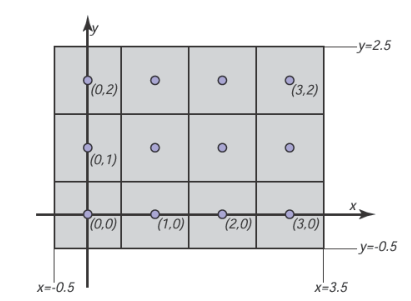
\includegraphics[width=1.0\textwidth]{3.10.png}
  \caption{一个拥有4个像素*3个像素的屏幕的坐标系。注意在部分API中$y$轴会指向下方。}
\end{figure}

一个平淡但重要的问题是像素在二维平面内如何定位。这只是一个约定俗成的问题,但创建一个一致的约定很重要!在本书中,光栅图像由一对$(i,j)$索引,指示像素的列$(i)$和行$(j)$,从左下角开始计数。如果图像具有$n_x$列、$n_y$行像素,则左下角的像素为$(0,0)$,右上角为像素$(n_x-1,n_y-1)$。我们需要二维实际屏幕坐标来指定像素位置。我们将像素的采样点放置在整数坐标处,如图3.10中的4 x 3屏幕所示。

\marginpar{
  \begin{center}
    \begin{note}\\
      在一些API和许多文件格式中,图片的行从上到下组织,因此$(0,0)$点在左上角。这是由于历史原因:模拟电视广播的行就是从顶端开始。
    \end{note}
  \end{center}
}

\marginpar{
  \begin{center}
    \begin{note}\\
      一些系统将坐标系移动了半个像素,以将采样点放置在整数之间的中间位置、将图像边缘放置在整数上。
    \end{note}
  \end{center}
}

图像的矩形区域具有宽度$n_x$和高度$n_y$,并且以此网格为中心,这意味着它延伸到每侧的最后一个采样点之外半个像素。所以$n_x \times n_y$图像的矩形域是:

\[
    R=[-0.5,n_x-0.5]\times [-0.5,n_y-0.5].
\]

同样,这些坐标只是约定,但稍后在实现相机和视图变换时记住它们非常重要。

\subsection{像素值}

到目前为止,我们已经用实数描述了像素的值,表示图像中某个点的强度(可能分别用于表示红色,绿色和蓝色)。这表明图像应该是一个由浮点数组成的阵列,其中每个像素存储一个(对于灰度或黑白图像)或三个(对于RGB彩色图像)32位浮点数。当需要其精度和值范围时,有时会使用这种格式,但是图像具有大量的像素,并且用于存储和传输图像的内存和带宽总是稀缺的。在这种格式下,仅一张1000万像素的照片就会消耗大约115MB的RAM。

\marginpar{
  \begin{center}
    \begin{note}\\
      为什么是115MB而不是120MB?
    \end{note}
  \end{center}
}

对于要直接显示的图像,需要的范围更小。虽然可能的光强度范围原则上是无限制的,但任何给定的设备都有一个明确的最大强度,所以在许多情况下,像素有一个有边界的范围是完全足够的,为了简单起见,通常取值为$[0,1]$。例如,8位图像的可能值是O,1/255,2/255,……,254/255,1。用浮点数存储的图像,允许很大的数值范围,通常被称为高动态范围(HDR)图像,以区别于固定范围或用整数存储的低动态范围(LDR)图像。关于高动态范围图像的技术和应用的深入讨论,详见第20章。

\marginpar{
  \begin{center}
    \begin{note}\\
      分母是255而非256,这很不雅观,但能准确表示0和1是很重要的。
    \end{note}
  \end{center}
}

此处有一些像素格式以及它们的代表性应用:
\begin{itemize}
  \item 1位灰度图像——文本和其他不需要中间灰度的图像(需要高分辨率)
  \item 8位RGB固定范围颜色(每个像素24位)——网络和电子邮件应用,消费者照片
  \item 8或10位固定范围RGB(每个像素24位或30位)——到计算机显示器的数码接口
  \item 12-14位固定范围RGB(每个像素36-42位)——专业摄影的原始相机图像
  \item 16位固定范围RGB(每个像素48位)——专业摄影与打印;用于固定范围图像处理的中间格式
  \item 16位固定范围灰度图像(每个像素16位)——放射学和医学图像
  \item 16位“半精度”浮点RGB——HDR图像;实时渲染的中间格式
  \item 32位浮点RGB——通用目的中间格式,用于HDR图像的软件渲染和处理。
\end{itemize}

减少用于存储每个像素的位数会导致图像中出现两种不同的伪影(artifact)类型(或人为引入的缺陷)。一、用固定范围的值对图像进行编码会产生裁剪(clipping),当其他比最大值更亮的像素被设置或裁剪为最大可表示的值。例如,一张阳光明媚的景物照片可能包括比白色表面亮得多的再反射;当图像被转换为固定范围显示时,这些反射会被剪掉(即使它们是由相机测量的)。第二,以有限的精度对图像进行编码会导致量化的伪影(quantization artifact),或带状现象(banding),当需要将像素值四舍五入到最接近的可表示值时,就会在强度或颜色上出现明显的跳跃。带状现象在动画和视频中特别隐蔽,在静止的图像中带状现象可能并不令人讨厌,但当它们来回移动时就变得非常明显。

\subsection{显示器强度与伽马(Gamma)}

所有的现代显示器都是使用数字输入作为一个像素的“值”,并将其转换为一个强度等级。真正的显示器在关闭时有一些非零强度,因为屏幕会反射一些光线。为了我们的目的,我们可以认为这是“黑色”,而显示器完全打开则是“白色”。我们假设对像素颜色的数字描述从0到1不等。黑色是0,白色是1,介于黑色和白色之间的灰色是0.5。请注意,这里的“一半”指的是来自像素的物理光量,而不是外观。人类对强度的感知是非线性的,这不会成为本讨论的一部分;更多内容详见第19章。

要在显示器上产生正确的图像,有两个关键问题必须了解。第一个问题是,显示器对于输入是非线性的。例如,如果你给显示器的三个像素输入0、0.5和1.0,显示的强度可能是0、0.25和1.0(关闭、四分之一全开和全开)。作为这种非线性的近似描述,显示器通常以$\gamma $(“gamma”)值为特征。这个值是下面公式中的自由度:
\begin{align}
  \text{显示强度}=\text{(最大强度)}a^\gamma
\end{align}
其中$a$是介于0和1之间的输入像素值。比如,如果一台显示器有2.0的伽马值,并且我们输入$a=0.5$,则显示强度是四分之一最大可能强度(因为$0.5^2=0.25$)。注意$a=0$映射到0强度、$a=1$映射到与$\gamma$值无关的最大强度。使用$\gamma$描述显示器的非线性度只是一个近似值;我们不需要很高的精度来估计设备的$\gamma$精度。衡量非线性度的一个很好的视觉方法是找到能产生介于黑白之间的中间强度的$a$值。这个$a$会如下所示:
\[
  \begin{aligned}
    0.5 = a^\gamma
  \end{aligned}
\]
如果我们能找到这样一个$a$,就能通过在两边取对数来推断出$\gamma$:
\[
  \begin{aligned}
    \gamma = \frac{\ln 0.5}{\ln a}
  \end{aligned}
\]

我们可以通过一个标准技术找到这个$a$,即在“输入$a$”的灰色像素正方形旁边显示一个黑白像素的棋盘图案(图3.11),然后要求用户调整$a$(例如用滑块),直到两边的平均亮度一致。当你从远处看这幅图时(如果你是近视眼,也可以不戴眼镜),当$a$产生的中间强度介于黑色和白色之间时,图的两边看起来差不多。这是因为模糊的棋盘混合了偶数的白色和黑色像素,所以整体效果是介于白色和黑色之间的统一颜色。

\marginpar{
  \begin{center}
    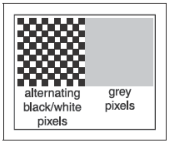
\includegraphics[width=0.25\textwidth]{3.11.png}
    \captionof{figure}{交替的黑、白像素在一段距离外看是介于黑色、白色之间的中间值。显示器的伽马值可通过找到一个看起来与黑白图案有相同强度的灰色值来推断出来。}
  \end{center}
}

一旦我们知道了$\gamma$,我们就可以对我们的输入进行伽马校正gamma correct),使$a=0.5$的值在显示时具有介于黑与白之间的中间强度。这是通过如下转换实现的;
\[
  \begin{aligned}
    a^{'} = a^{\frac{1}{\gamma } }
  \end{aligned}
\]
当把以上公式代入等式3.1,我们得到了:
\[
  \begin{aligned}
    \text{显示强度} = (a^{'})^\gamma = (a^{\frac{1}{\gamma}})\text{(最大强度)} = a\text{(最大强度)}
  \end{aligned}
\]

\marginpar{
  \begin{center}
    \begin{note}\\
      使用模拟接口的显示器在水平方向上更难迅速改变强度,因此水平黑白线的效果比棋盘格更好。
    \end{note}
  \end{center}
}

实数显示器的另一个重要特征是,它们采取量化的输入值。因此,虽然我们可以在浮点范围$[0,1]$内操作强度,但显示器的详细输入是一个固定大小的整数。这个整数最常见的范围是0-255,可以用8比特的存储空间来保存。这意味着$a$的可用值不是$[O,1]$中的任何数值,而是:
\[
  \begin{aligned}
    \text{a的可能值} = \left\{ \frac{0}{255},\frac{1}{255},\frac{2}{255},……,\frac{254}{255},\frac{255}{255}\ \right\}
  \end{aligned}
\]
这意味着可能的显示强度值近似于以下值:
\[
  \begin{aligned}
    \left\{ M(\frac{0}{255})^\gamma ,M(\frac{1}{255})^\gamma ,M(\frac{2}{255})^\gamma ,……,M(\frac{254}{255})^\gamma ,M(\frac{255}{255})^\gamma \right\}
  \end{aligned}
\]
其中$M$是最大强度。在需要控制确切强度的应用中,我们必须实际测量256种可能的强度,并且这些强度在屏幕上的不同点可能不同,特别是对于CRT设备。它们也可能随视角而变化。幸运的是,很少有应用需要如此精确的校准。

\section{RGB颜色}

\marginpar{
  \begin{center}
    \begin{note}\\
      在小学你可能学习到了红、绿、蓝是三原色,并且例如,黄色+蓝色=绿色。这是减色混合,这与显示器中发生的更熟悉的加色混合有根本的不同。
    \end{note}
  \end{center}
}

大多数计算机图形图像是根据红-绿-蓝(RGB)颜色定义的。RGB颜色是一个简单的空间,允许直接转换给大多数计算机屏幕的控制。在本节中,我们会从用户角、以便利操作为目标讨论RGB颜色。第18章对颜色进行了更全面的讨论,但是RGB色彩空间的机制将使我们能够使用大多数图形学程序。RGB色彩空间的基本思想是通过混合三个主要光源来显示颜色:一个红色、一个绿色和一个蓝色。灯光以加色方式混合。

在RGB加色混合中我们得到了(图3.12):
\marginpar{
  \begin{center}
    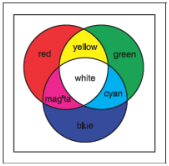
\includegraphics[width=0.25\textwidth]{3.12.png}
    \captionof{figure}{红、绿、蓝三色的加色混合规则。}
  \end{center}
}
\[
  \begin{aligned}
    \text{红色} + \text{绿色}             & = \text{黄色}, \\
    \text{绿色} + \text{蓝色}             & = \text{青色}, \\
    \text{蓝色} + \text{红色}             & = \text{品红}, \\
    \text{红色} + \text{绿色} + \text{蓝色} & = \text{白色}。
  \end{aligned}
\]
“青色”是一种蓝绿色,“品红”是一种紫色。

如果我们被允许将主灯从完全关闭(用像素值0表示)调至完全打开(用1表示),我们就可以创造出所有可以在RGB显示器上显示的颜色。红色、绿色和蓝色的像素值创建了一个三维的RGB颜色立方体,它有一个红色、一个绿色和一个蓝色轴。轴的最小坐标值范围是0到1。图3.13是彩色立方体的图示。

\begin{figure}[htb]
  \centering
  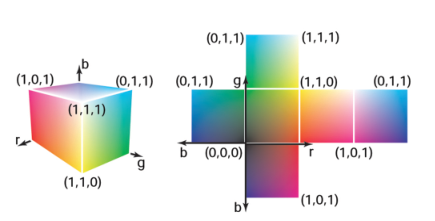
\includegraphics[width=1.0\textwidth]{3.13.png}
  \caption{RGB颜色立方体和其完全展开的面。任何RGB颜色都是立方体上的一个点。}
\end{figure}

立方体角落的颜色是:
\[
  \begin{aligned}
    \text{黑色} & = (0,0,0), \\
    \text{红色} & = (1,0,0), \\
    \text{绿色} & = (0,1,0), \\
    \text{蓝色} & = (0,0,1), \\
    \text{黄色} & = (1,1,0), \\
    \text{品红} & = (1,0,1), \\
    \text{青色} & = (0,1,1), \\
    \text{白色} & = (1,1,1).
  \end{aligned}
\]

实际的RGB等级通常以量化的形式给出,就像第3.2.2节中讨论的灰阶(grayscale)一样。每个分量都用一个整数来指定。这些整数最常见的大小是每个分量一个字节,所以RGB的三个分量都是0到255之间的整数。这三个整数加起来占了三个字节,也就是24位。因此,一个拥有“24位色彩”的系统,三原色中的每一种都有256个可能的级别。第3.2.2节中讨论的伽玛校正问题也分别适用于RGB的每个分量。

\section{阿尔法合成}

通常情况下,我们只想部分地覆盖一个像素的内容。一个典型的例子发生在合成中,我们有一个背景,想在上面插入一个前景图像。对于前景中不透明的像素,我们只需替换背景像素。对于完全透明的前景像素,我们不改变背景像素。对于部分透明的像素,必须小心谨慎。当前景物体有部分透明区域时,如玻璃,就会出现部分透明像素。但是,前景和背景必须混合的最常见的情况是,前景物体只覆盖了部分像素,要么是在前景物体的边缘,要么是有子像素孔,如远处的树叶之间。

如果我们想在背景物体上混合一个前景物体,最重要的信息是像素覆盖率(pixel coverage),它告诉我们前景层所覆盖的像素的比例。我们可以称这个分数为$\alpha $。如果我们想要将一个前景色$c_f$合成到背景色$c_b$上,而且被前景覆盖的像素比例是$\alpha $,那我们就可以用下面这个公式:
\begin{equation}
  c = \alpha c_f + (1 - \alpha )c_b
\end{equation}
对于一个不透明的前景层,这个公式的解释是前景物体覆盖了像素矩形内的比例为$\alpha $的区域,而背景物体覆盖了剩余的区域,也就是比例为$(1-\alpha )$的区域。对于透明层(想想在玻璃或描图纸上画的图像,使用半透明的油漆),这个公式的解释是前景层阻挡了从背景透过来的那部分光线(比例为$(1-\alpha )$),并贡献了一部分(比例为$\alpha $)自己的颜色来替代被移除的部分。图3.14显示了一个使用公式3.2的例子。

\marginpar{
  \begin{center}
    \begin{note}\\
      由于前景层和背景层的权重相加为1,如果前景层和背景层的颜色相同,颜色就不会改变。
    \end{note}
  \end{center}
}

\begin{figure}[htb]
  \centering
  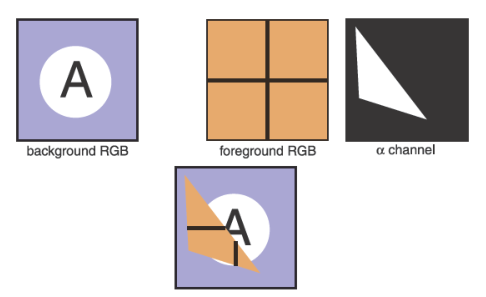
\includegraphics[width=0.6\textwidth]{3.14.png}
  \caption{上图是一个使用公式3.2的合成示例。前景图像在被放在背景图像之上之前,实际上是被$\alpha $通道裁剪过的。合成结果显示在底部。}
\end{figure}

一个图像中所有像素的$\alpha $值可能被存储在一个单独的灰度图像中,然后被称为阿尔法遮罩(alpha mask)或透明度遮罩(transparency mask)。或者信息可以被存储为RGB图像中的第四个通道,在这种情况下,它被称为阿尔法通道(alpha channel),因此图像可以被称为RGBA图像。
对于8位图像,每个像素占32位,这在许多计算机架构中是一个大小方便的数据块。

尽管公式3.2常被使用,但有一些情况下$\alpha $会有其他不同的用法。(Porter \& Duff,1984)。

\subsection{图像存储}

大多数RGB图像格式的红、绿、蓝三色通道各使用8比特。这样一来,一张100万像素的图像大约需要3兆字节的原始信息。为了减少存储需求,大多数图像格式允许某种压缩。在高层次上,这种压缩是无损(lossless)的或有损(lossy)的。在无损压缩中,没有信息被丢弃,而在有损系统中,一些信息会不可恢复地丢失。流行的图像存储格式包括:
\begin{itemize}
  \item \textcolor{lightgreen}{jpeg.} 这种有损格式是根据人类视觉系统的阈值来压缩图像块。这种格式对自然图像很有效。
  \item \textcolor{lightgreen}{tiff.} 这种格式最常用于保存二进制图像或无损压缩的8位或16位RGB,尽管还有许多其他选择。
  \item \textcolor{lightgreen}{ppm.} 这种非常简单的无损、未压缩的格式最常用于8位RGB图像,尽管还有许多其他选择。
  \item \textcolor{lightgreen}{png.} 这是一套无损格式,有一套很好的开放源码管理工具。
\end{itemize}
由于压缩和变体的原因,为图像编写输入/输出例程可能会涉及到。幸运的是,人们通常可以依靠库中的例程来读写标准文件格式。对于快速、肮脏的应用来说,简单的价值高于效率,一个简单的选择是使用原始的PPM文件,这通常可以简单地通过将存储在内存中的图像的数组转储到一个文件中来编写,并在头部追加适当的头文件。

\section{FAQ}

\subsection{\textcolor{lightgreen}{为什么他们不把显示器做成线性的,而避免所有这些伽马业务?}}

理想情况下,显示器的256种可能的强度看起来应该是均等分隔的的,而不是按照能量线性分隔。因为人类对强度的感知本身就是非线性的,伽玛值在1.5和3之间(取决于观看条件),会使强度在主观上近乎均匀。这样一来,伽玛就成了一种特性。否则,制造商会把显示器做成线性的。

\section{练习}

通过拍摄自然图像(最好是扫描的照片,而不是可能已经应用了拜尔马赛克的数码照片),并创建一个由红/绿/蓝通道交错组成的灰度图像,来模拟从拜尔马赛克获得的图像。这模拟了数码相机的原始输出。现在从该输出创建一个真正的RGB图像,并与原始图像进行比较。
